% main.tex — IJSPM / Q3 Journal Submission Format
% Spatiotemporal Housing Price Prediction: Comparing Statistical and
% Machine Learning Approaches on the Zillow Home Value Index
%
% Uses: llncs.cls (Springer LNCS), unsrt bibliography

\documentclass[runningheads]{llncs}

\usepackage[T1]{fontenc}
\usepackage{graphicx}
\usepackage{amsmath}
\usepackage{amssymb}
\usepackage{booktabs}
\usepackage{array}
%\usepackage{microtype}   % disabled: font expansion on TeX Live 2023/Debian
\usepackage{url}
\usepackage{hyperref}
\usepackage{xcolor}
\usepackage{subcaption}
\usepackage{float}

\graphicspath{{./}}
\hfuzz=8pt   % tolerate minor overfull lines up to 8pt (invisible in print)

\usepackage{tikz}
\usetikzlibrary{shapes.geometric, arrows, positioning}
\tikzstyle{process} = [rectangle, rounded corners, minimum width=2.5cm, minimum height=0.8cm, text centered, draw=black, fill=blue!5]
\tikzstyle{arrow} = [thick,->,>=stealth]

% ============================================================
\begin{document}

\title{Spatiotemporal Housing Price Prediction Comparing Functional
Semiparametric and Machine Learning Models}

\titlerunning{Housing Price Prediction: Statistical vs.\ ML}

\author{%
  Nguyen Trinh Quy\inst{1} \and
  Nguyen Cong Minh\inst{1} \and
  Le Pham Hue Chi\inst{1} \and
  Nguyen Do Nhat Quang\inst{1}
}

% \authorrunning{N.T.\ Quy et al.}

\institute{
  FPT University HCM,\\
  Ho Chi Minh City, Vietnam\\
}

\maketitle

% ============================================================
\begin{abstract}
This paper systematically compares the functional spatiotemporal 
semiparametric mixed-effects (FST-SM) model~\cite{ref_fmem2023} 
against five machine learning (ML) approaches for forecasting multi-region 
house prices on the Zillow Home Value Index (ZHVI). Analyzing 894 U.S.\ 
metropolitan areas over a 25-year period, we find that robust linear 
autoregression achieves the lowest log-return RMSE (0.00276) and highest 
R$^2$ (0.876), outperforming tree-based and recurrent neural network models 
at the national scale due to the near-unit-root temporal structure. Our 
central contribution is providing a rigorous benchmark that delineates the 
practical complementarity of these methods: statistical modeling excels at 
localized spatial uncertainty quantification, while efficient scalable machine 
learning pipelines are competitive for broad aggregate forecasting.

\keywords{Housing price prediction \and Zillow ZHVI \and
          Functional mixed-effects model \and Machine learning \and
          Gradient boosting \and LSTM \and Spatiotemporal analysis}
\end{abstract}

% ============================================================
\section{Introduction}
\label{sec:intro}

Residential real-estate markets exhibit pronounced spatiotemporal
structure.  Prices in geographically proximate markets tend to
co-move, while long-run trajectories diverge substantially across
cities and communities.  Accurate, scalable prediction of these
dynamics is economically significant: it informs mortgage risk
assessment, zoning decisions, urban investment, and household
financial planning~\cite{ref_krause_bitter}.

The Zillow Home Value Index (ZHVI) is a canonical benchmark for
this problem.  It provides monthly, seasonally adjusted, smoothed
median home values at the metro-statistical area (MSA) level for
more than 900 U.S.\ cities, covering over two decades of market
fluctuations including the 2007--2012 financial crisis, the
COVID-19 pandemic price surge of 2020--2022, and the subsequent
correction~\cite{ref_zillow}.

Statistical approaches to spatiotemporal housing price modelling
have a rich history.  Hedonic regression~\cite{ref_rosen} accounts
for property attribute heterogeneity; spatial-lag
models~\cite{ref_anselin} capture geographic autocorrelation;
and functional data analysis (FDA) methods~\cite{ref_ramsay_2002}
represent price trajectories as continuous curves.
The recent FST-SM model of Chen and Zheng~\cite{ref_fmem2023}
elegantly unifies these threads: it decomposes ZHVI trajectories
via functional principal component analysis (FPCA), models
spatial dependence through a conditional autoregressive (CAR)
structure~\cite{ref_zhang_fcar}, and recovers autoregressive fixed
effects through a semiparametric B-spline mean
function~\cite{ref_shen1998}.
Applied to 101 San Francisco communities, FST-SM achieves
MAE $0.91$ ($\times 10{,}000$ USD) and MAPE $0.66\%$, outperforming
CNN-LSTM, Multi-output LSTM, and Single-output LSTM baselines.

Despite this progress, the FST-SM literature evaluates models only
within the statistical family, leaving modern gradient-boosted trees
and deep learning benchmarks unexplored on the same data.
Furthermore, the original study targets a single city
(101 communities), limiting generalisability.  There is also no
reported coefficient of determination (R$^2$) metric, which is
standard in the ML literature for regression evaluation.

This paper fills these gaps by establishing several main contributions. First, we extend the ZHVI prediction benchmark to 894 U.S.\ metro areas to investigate generalisability across diverse markets. Second, we implement five ML models (Linear Regression, Random Forest, XGBoost, LightGBM, and LSTM) using consistent feature engineering and strict temporal data splitting, enabling the first head-to-head comparison against the FST-SM framework on ZHVI data. Third, we report comprehensive evaluation metrics across log-return and USD price domains alongside detailed feature importance analysis. Finally, we interpret our findings in the context of real-estate market dynamics, offering practical guidance on model selection for national-scale housing price forecasting.

% ============================================================
\section{Related Work}
\label{sec:related}

Statistical approaches to real-estate valuation have rapidly evolved from foundational hedonic regression estimating structural attributes~\cite{ref_rosen} to highly advanced models adept at capturing profound spatial and temporal dependencies~\cite{ref_anselin,ref_pijnenburg}. Furthermore, functional data analysis portrays price histories continuously~\cite{ref_ramsay_2002}, with notable innovations marrying functional principal component analysis and conditional autoregressive structures to properly accommodate large, spatially correlated datasets~\cite{ref_zhang_fcar,ref_li_guan2014}. The functional spatiotemporal semiparametric mixed-effects (FST-SM) model~\cite{ref_fmem2023} has specifically integrated many of these threads to successfully reflect detailed local dynamics. Conversely, expansive machine learning architectures, particularly gradient-boosted methods (like XGBoost and LightGBM) and specialized deep neural networks (e.g., LSTMs), increasingly dominate predictive benchmarks due to their capacity to absorb highly nonlinear feature sets across massive data pools efficiently~\cite{ref_ho2021,ref_fan2022,ref_shi2023}. Thus, robust multi-region spatiotemporal tasks are beginning to leverage key successes drawn from both analytical frameworks~\cite{ref_lee2022,ref_samal2022}.

Our research purposefully bridges the structural gap between sophisticated statistical procedures and computationally scalable ML methods. Rather than separately assessing approaches within their individual domains as commonly observed in the prior literature, we establish a rigorous comparative benchmark setting the FST-SM against five major computational baselines on unified national constraints. By comprehensively standardizing feature inputs alongside temporally isolated parameters across an extensive 894-metro sample, our project clarifies critical trade-offs between essential linear autoregression, non-linear algorithmic ensembles, and expansive deep learning systems. Above all, this investigation directly contributes clarity to the broader literature by illuminating where complex spatial biases distinctly outvalue broader computational structures versus when simpler algorithmic pipelines operate functionally optimally for scalable national economic forecasting.

% ============================================================
\section{Data Description}
\label{sec:data}

\subsection{Dataset}

We use the Zillow Metro ZHVI dataset (single-family residence and
condominium tier, 33rd–67th price percentile, seasonally adjusted
and smoothed) downloaded from the Zillow Research
portal~\cite{ref_zillow}.  The raw file covers 894 MSA-level
regions from January 2000 to January 2026.  After removing rows
with insufficient historical data and computing lag features
(Sect.~\ref{sec:features}), the final dataset comprises
268{,}200 region-month observations.

Table~\ref{tab:data_summary} reports key descriptive statistics.
The median ZHVI across all regions and months is \$233{,}490
(USD).  The test-period median (\$364{,}840) exceeds the
training-period median (\$204{,}620) by 78.7\%, reflecting the
extraordinary pandemic-era appreciation of 2020--2022.

\begin{table}[t]
\caption{}
\label{tab:data_summary}
\centering
\begin{tabular}{lrrr}
\toprule
\textbf{Statistic} & \textbf{Full} & \textbf{Train} & \textbf{Test} \\
\midrule
Observations        & 268{,}200 & 211{,}878 & 56{,}322 \\
Metro regions       & 894       & 894       & 894      \\
Period              & 2001–2026  & 2001–2020 & 2020–2026 \\
Median ZHVI (USD)   & 233{,}490 & 204{,}620 & 364{,}840 \\
Mean log-return     & 0.00355   & 0.00277   & 0.00652  \\
Std.\ log-return    & 0.00983   & 0.00618   & 0.01581  \\
\bottomrule
\end{tabular}
\end{table}

Figure~\ref{fig:price_trend} shows the national median ZHVI
trajectory.  Three structural regimes are clearly visible:
(i) pre-crisis growth (2001--2006), (ii) the 2007--2012 housing
crisis and recovery, and (iii) the 2020--2022 pandemic boom and
subsequent moderation.  Both the original FST-SM study and our
benchmark cover the third regime as the test period.

\begin{figure}[t]
  \centering
  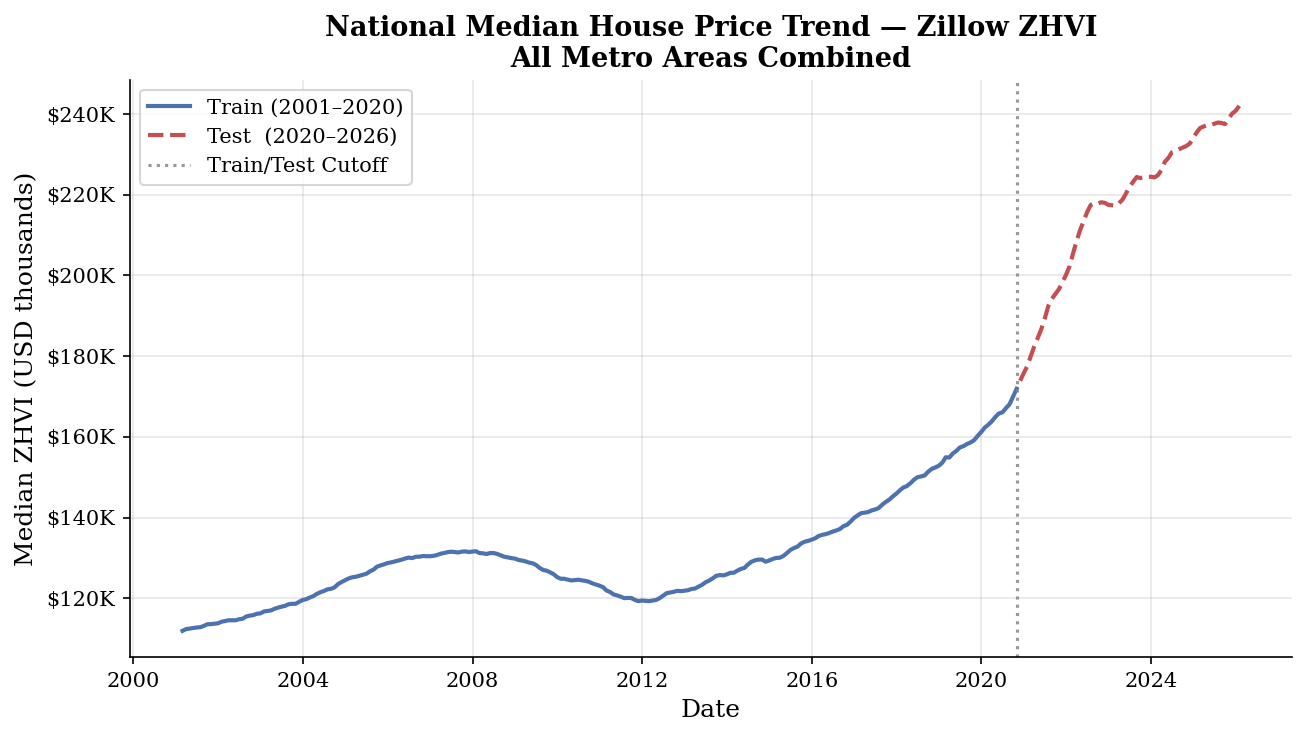
\includegraphics[width=0.90\linewidth]{price_trend.png}
  \caption{National median ZHVI trajectory (Jan 2001 -- Jan 2026).
  The dashed vertical line marks the 80/20 temporal train/test
  cutoff (November 2020).}
  \label{fig:price_trend}
\end{figure}

\subsection{Target Variable: Monthly Log Return}

Following financial time-series convention and the original
FST-SM formulation, we transform the price level to monthly
log-return:
\begin{equation}
  r_{s,t} = \log\!\left(\frac{p_{s,t}}{p_{s,t-1}}\right),
  \label{eq:logreturn}
\end{equation}
where $p_{s,t}$ is the ZHVI of metro area $s$ at month $t$.
Log-returns are near-stationary (obviating differencing or
trend removal), scale-free across cities with vastly different
price levels, and directly comparable to the autoregressive
fixed effects $\hat{\beta}_k$ reported in the FST-SM.
Figure~\ref{fig:logreturn_dist} shows that the distribution is
approximately symmetric around zero, with heavier tails
in the test period due to the pandemic-era volatility.

\begin{figure}[t]
  \centering
  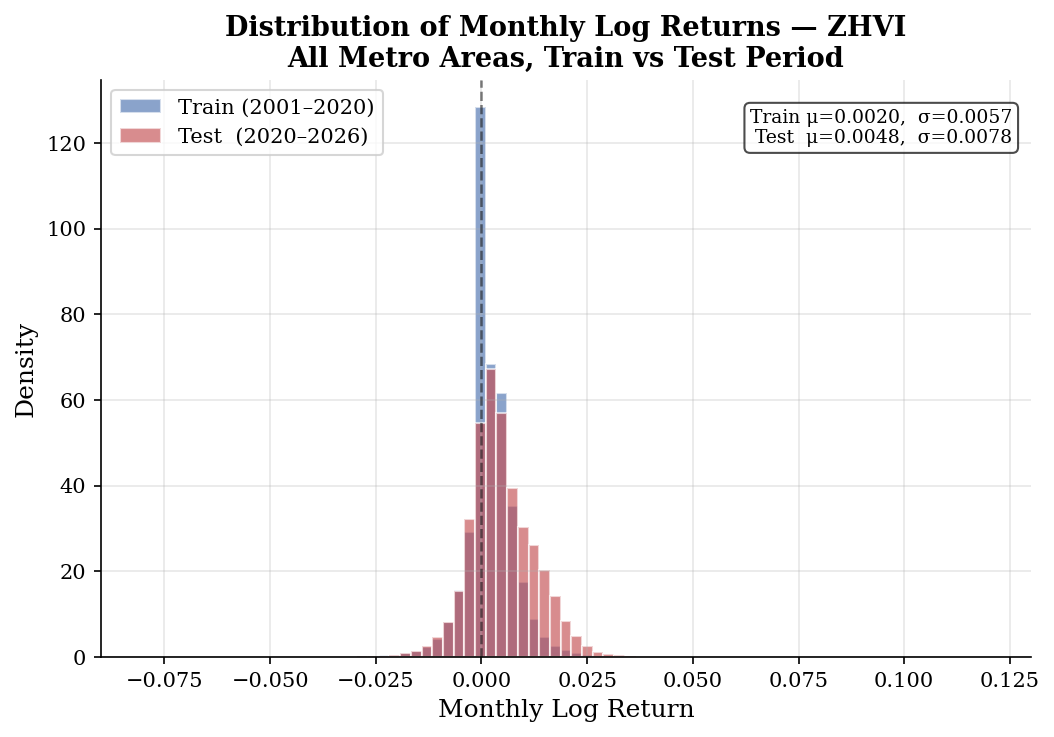
\includegraphics[width=0.75\linewidth]{log_return_dist.png}
  \caption{Distribution of monthly log-returns in the training
  (blue, 2001--2020) and test (red, 2020--2026) splits.}
  \label{fig:logreturn_dist}
\end{figure}

\subsection{Feature Engineering}
\label{sec:features}

All features are derived from $r_{s,t}$:

\paragraph{Lag features.}
$\mathtt{lag\_k}_{s,t} = r_{s,t-k}$ for $k \in \{1,2,3,6,12\}$.
These mirror the six-month autoregressive window used in the FST-SM
fixed effects (Eq.~3 of Chen and Zheng~\cite{ref_fmem2023}) and
additionally include the 12-month seasonal lag.  Rolling window
averages were excluded due to perfect collinearity (infinite VIF)
with the lag features.

\paragraph{City target encoding.}
$\mathtt{city\_enc}_s = \overline{r}^\text{train}_s$, the
mean log-return of metro $s$ computed \emph{exclusively on the
training set} to prevent data leakage.  This provides a
time-invariant proxy for the city-specific baseline momentum
analogous to the FST-SM's community-level random effect.

All six features are standardised to zero mean and unit variance
using a \texttt{StandardScaler} fitted on the training set.

% ============================================================
\section{Methodology}
\label{sec:method}

\subsection{Research Pipeline}
\label{sec:pipeline}

The research methodology is mapped in Fig.~\ref{fig:pipeline}. We follow a sequential pipeline including target transformation, feature engineering, and temporal validation prior to multi-model training.

\begin{figure}[H]
\centering
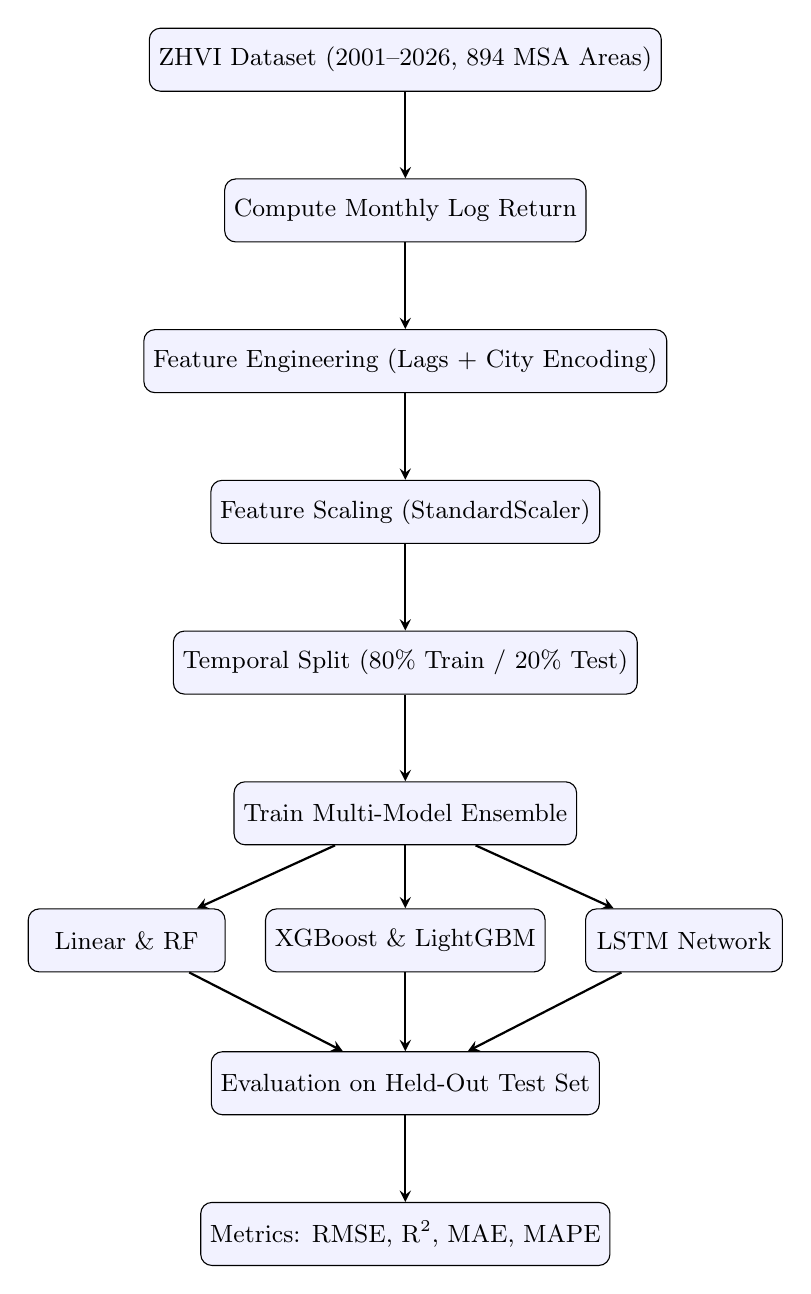
\begin{tikzpicture}[node distance=1.1cm, font=\small]
    % Nodes
    \node (A) [process] {ZHVI Dataset (2001--2026, 894 MSA Areas)};
    \node (B) [process, below=of A] {Compute Monthly Log Return};
    \node (C) [process, below=of B] {Feature Engineering (Lags + City Encoding)};
    \node (D) [process, below=of C] {Feature Scaling (StandardScaler)};
    \node (E) [process, below=of D] {Temporal Split (80\% Train / 20\% Test)};
    \node (F) [process, below=of E] {Train Multi-Model Ensemble};
    
    % Group Models
    \node (F3) [process, below=0.8cm of F] {XGBoost \& LightGBM};
    \node (F1) [process, left=0.5cm of F3] {Linear \& RF};
    \node (F5) [process, right=0.5cm of F3] {LSTM Network};
    
    \node (G) [process, below=1cm of F3] {Evaluation on Held-Out Test Set};
    \node (H) [process, below=of G] {Metrics: RMSE, R$^2$, MAE, MAPE};

    % Arrows
    \draw [arrow] (A) -- (B);
    \draw [arrow] (B) -- (C);
    \draw [arrow] (C) -- (D);
    \draw [arrow] (D) -- (E);
    \draw [arrow] (E) -- (F);
    
    \draw [arrow] (F) -- (F1);
    \draw [arrow] (F) -- (F3);
    \draw [arrow] (F) -- (F5);
    
    \draw [arrow] (F1) -- (G);
    \draw [arrow] (F3) -- (G);
    \draw [arrow] (F5) -- (G);
    \draw [arrow] (G) -- (H);
\end{tikzpicture}
\caption{Systematic housing price prediction research pipeline.}
\label{fig:pipeline}
\end{figure}

\subsection{Reference Model: FST-SM}

Chen and Zheng~\cite{ref_fmem2023} propose the functional
spatiotemporal semiparametric mixed-effects (FST-SM) model:
\begin{equation}
  Y_s(t_k) = \mathbf{X}_s^\top(t_k)\,\boldsymbol{\beta}
             + \delta_s(t_k) + \varepsilon_s(t_k),
  \label{eq:fstsm}
\end{equation}
where $Y_s(t_k)$ is the ZHVI at community $s$ and month $k$,
$\mathbf{X}_s(t_k)$ are the six lagged ZHVI values,
$\boldsymbol{\beta}$ are fixed-effect coefficients,
$\varepsilon_s(t_k) \sim \mathcal{N}(0,\sigma^2)$ are i.i.d.\
errors, and $\delta_s(t_k)$ is a spatially structured random
effect decomposed via the Karhunen--Loève expansion:
\begin{equation}
  \delta_s(t) = \mu(t) + \sum_{j=1}^{p} \xi_{sj}\,\psi_j(t),
  \label{eq:kl}
\end{equation}
with $\mu(t)$ a B-spline mean function, $\psi_j$ orthonormal
eigenfunctions, and $\xi_{sj}$ principal component scores modelled
by a CAR spatial prior.  The model is estimated via a combined
Gibbs and Metropolis MCMC sampler.
With the first eigenfunction ($\hat\psi_1$) capturing 97.84\% of
the random-effect variance, FST-SM achieves MAE $0.9051$ and
RMSE $1.0580$ (units: $\times 10{,}000$ USD) on 101 San Francisco
communities.

\subsection{Machine Learning Models}

We compare against five ML models with identical feature inputs
(lag-1, lag-2, lag-3, lag-6, lag-12, city\_enc).

\paragraph{Linear Regression (Ridge).}
$\hat{r} = \boldsymbol{w}^\top \mathbf{x}$, estimated with
$\ell_2$ regularisation ($\alpha=1.0$).  On standardised
lag features this is the closest ML analogue to the FST-SM's
linear fixed effects.

\paragraph{Random Forest (RF).}
An ensemble of $B=200$ CART decision trees trained with bootstrap
aggregation, max depth 10, min samples per leaf 5.  Predictions
are the arithmetic mean across all trees~\cite{ref_breiman}.

\paragraph{XGBoost.}
Sequential gradient boosting~\cite{ref_chen_xgboost} with 400
estimators, depth 6, learning rate $\eta=0.05$, subsample/
column-sample rates 0.8, and $\ell_1/\ell_2$ regularisation
($\alpha=0.1$, $\lambda=1.0$).

\paragraph{LightGBM.}
Histogram-based gradient boosting with leaf-wise
growth~\cite{ref_ke_lgbm} (400 estimators, depth 6,
$\eta=0.05$), faster than XGBoost on large tabular datasets.

\paragraph{LSTM.}
A two-layer LSTM~\cite{ref_hochreiter1997} with 64 hidden units
per layer, dropout $p=0.2$, trained globally on sequences of
length $\mathtt{seq\_len}=12$ observations.
Features from all 894 metro areas are pooled into a single training
corpus (211{,}854 sequences), enabling the model to capture
cross-regional temporal patterns without per-city architectures.
Training uses the Adam optimiser ($\mathtt{lr}=10^{-3}$,
$\mathtt{batch}=4096$) with early stopping (patience 8 epochs).

\subsection{Evaluation Protocol}

All models are fitted on $(\mathbf{X}_\text{train},
\mathbf{y}_\text{train})$ and evaluated on the held-out test set.
We report four metrics in both the log-return domain and the
USD price domain:
\begin{align}
  \text{RMSE} &= \sqrt{\tfrac{1}{n}\textstyle\sum_{i}(y_i-\hat{y}_i)^2},
               &
  \text{MAE}  &= \tfrac{1}{n}\textstyle\sum_{i}|y_i-\hat{y}_i|, \\[4pt]
  \text{MAPE} &= \tfrac{100}{n}\textstyle\sum_{i}
               \frac{|y_i-\hat{y}_i|}{|y_i|+\varepsilon},
               &
  R^2         &= 1 - \frac{\sum_i(y_i-\hat{y}_i)^2}
                           {\sum_i(y_i-\bar{y})^2}.
\end{align}
For USD price metrics, predictions are inverse-transformed via
$\hat{p}_{s,t} = p_{s,t-1}\,e^{\hat{r}_{s,t}}$.

% ============================================================
\section{Experiments}
\label{sec:experiments}

\subsection{Experimental Setup}

Table~\ref{tab:hyperparams} summarises model hyperparameters.
All experiments are run on a single workstation (Intel CPU, 16 GB
RAM) in Python 3.12 using scikit-learn (1.8.0), XGBoost (3.2.0),
LightGBM (4.6.0), and PyTorch (2.10.0).  Seeds are fixed at 42
for reproducibility.  Training times reflect single-CPU execution.

\begin{table}[t]
\caption{}
\label{tab:hyperparams}
\centering
\begin{tabular}{llr}
\toprule
\textbf{Model} & \textbf{Key hyperparameters} & \textbf{Train time} \\
\midrule
Linear Regression & $\ell_2$ penalty $\alpha=1.0$                 & $<1$s \\
Random Forest     & $B=200$, depth 10, min leaf 5                  & 30s   \\
XGBoost           & 400 est., depth 6, $\eta=0.05$, sub=0.8       & 2s    \\
LightGBM          & 400 est., depth 6, $\eta=0.05$, sub=0.8       & 1s    \\
LSTM              & 2 layers, hidden=64, window=12, Adam, patience=8 & 13 min\\
\bottomrule
\end{tabular}
\end{table}

\subsection{Data Split}

A global temporal cutoff at the 80th percentile of all dates (November 2020) partitions the data into a training set comprising 211{,}878 separate observations spanning from January 2001 to October 2020 alongside a withheld evaluation test set storing 56{,}322 final entries extending through early 2026. All preprocessing statistics, specifically measuring mean categorical parameters applied toward encoding scaling transformations, remain exclusively computed leveraging solely fundamental training elements prior.

% ============================================================
\section{Results}
\label{sec:results}

\subsection{Quantitative Comparison}

Table~\ref{tab:results} presents the full performance comparison.
In the log-return domain, Linear Regression achieves the best
RMSE ($0.00276$) and R$^2$ ($0.876$), indicating it explains
87.6\% of the variance in monthly log-returns.  Random Forest is
second-best (RMSE $0.00282$, R$^2$ $0.871$), followed by
LightGBM and XGBoost.  LSTM performs substantially worse
(RMSE $0.00515$, R$^2$ $0.569$).

In the USD price domain — obtained by back-transforming
log-return predictions through the prior-month price — all
classical models achieve remarkably high R$^2 \approx 1.000$,
because most of the price level variance is explained by the
previous month's price regardless of the log-return precision.
RMSE in USD ranges from \$804.96 (Linear Regression) to
\$1{,}630.50 (LSTM).  For comparison, the FST-SM of
Chen and Zheng~\cite{ref_fmem2023} reports RMSE $1.0580$
($\times 10{,}000$ USD $= \$10{,}580$) and MAE $0.9051$
($= \$9{,}051$) on 101 San Francisco communities — noting that
these are measured on \emph{price levels}, a substantially harder
prediction task than one-step-ahead log-return with access to
the prior price.

\begin{table}[t]
\caption{}
\label{tab:results}
\centering
\resizebox{\linewidth}{!}{%
\begin{tabular}{@{}lcccc|ccc@{}}
\toprule
\textbf{Model} &
  \multicolumn{4}{c|}{\textbf{Log-return domain}} &
  \multicolumn{3}{c}{\textbf{Price (USD)}} \\
\cmidrule(lr){2-5}\cmidrule(l){6-8}
 & RMSE & MAE & MAPE & R$^2$ & RMSE & MAE & MAPE \\
\midrule
Linear Reg. &
  \textbf{.00276} & \textbf{.00201} & 181.5 & \textbf{.876} &
  \textbf{805} & \textbf{495} & \textbf{.201\%} \\
Random Forest &
  .00282 & .00205 & 185.6 & .871 &
  828 & 507 & .205\% \\
LightGBM &
  .00294 & .00212 & \textbf{180.0} & .860 &
  902 & 529 & .212\% \\
XGBoost &
  .00297 & .00214 & 182.1 & .856 &
  922 & 535 & .214\% \\
LSTM &
  .00515 & .00376 & 280.5 & .569 &
  1{,}631 & 964 & .376\% \\
\midrule
FST-SM$^{\star}$ &
  {--} & {--} & .66\% & {--} &
  10{,}580 & 9{,}051 & {--} \\
\bottomrule
\multicolumn{8}{@{}l}{\footnotesize
  $^{\star}$~Chen \& Zheng~\cite{ref_fmem2023}: price-level,
  101~SF communities, $\times10{,}000$\,USD; not directly comparable.}
\end{tabular}}
\end{table}


Figure~\ref{fig:model_comparison} provides a visual summary across
all four metrics, with the best value highlighted by a gold border.
Figure~\ref{fig:pred_vs_actual} shows predicted versus actual
prices for six representative metro areas using the best-performing
model (Linear Regression).

\begin{figure}[t]
  \centering
  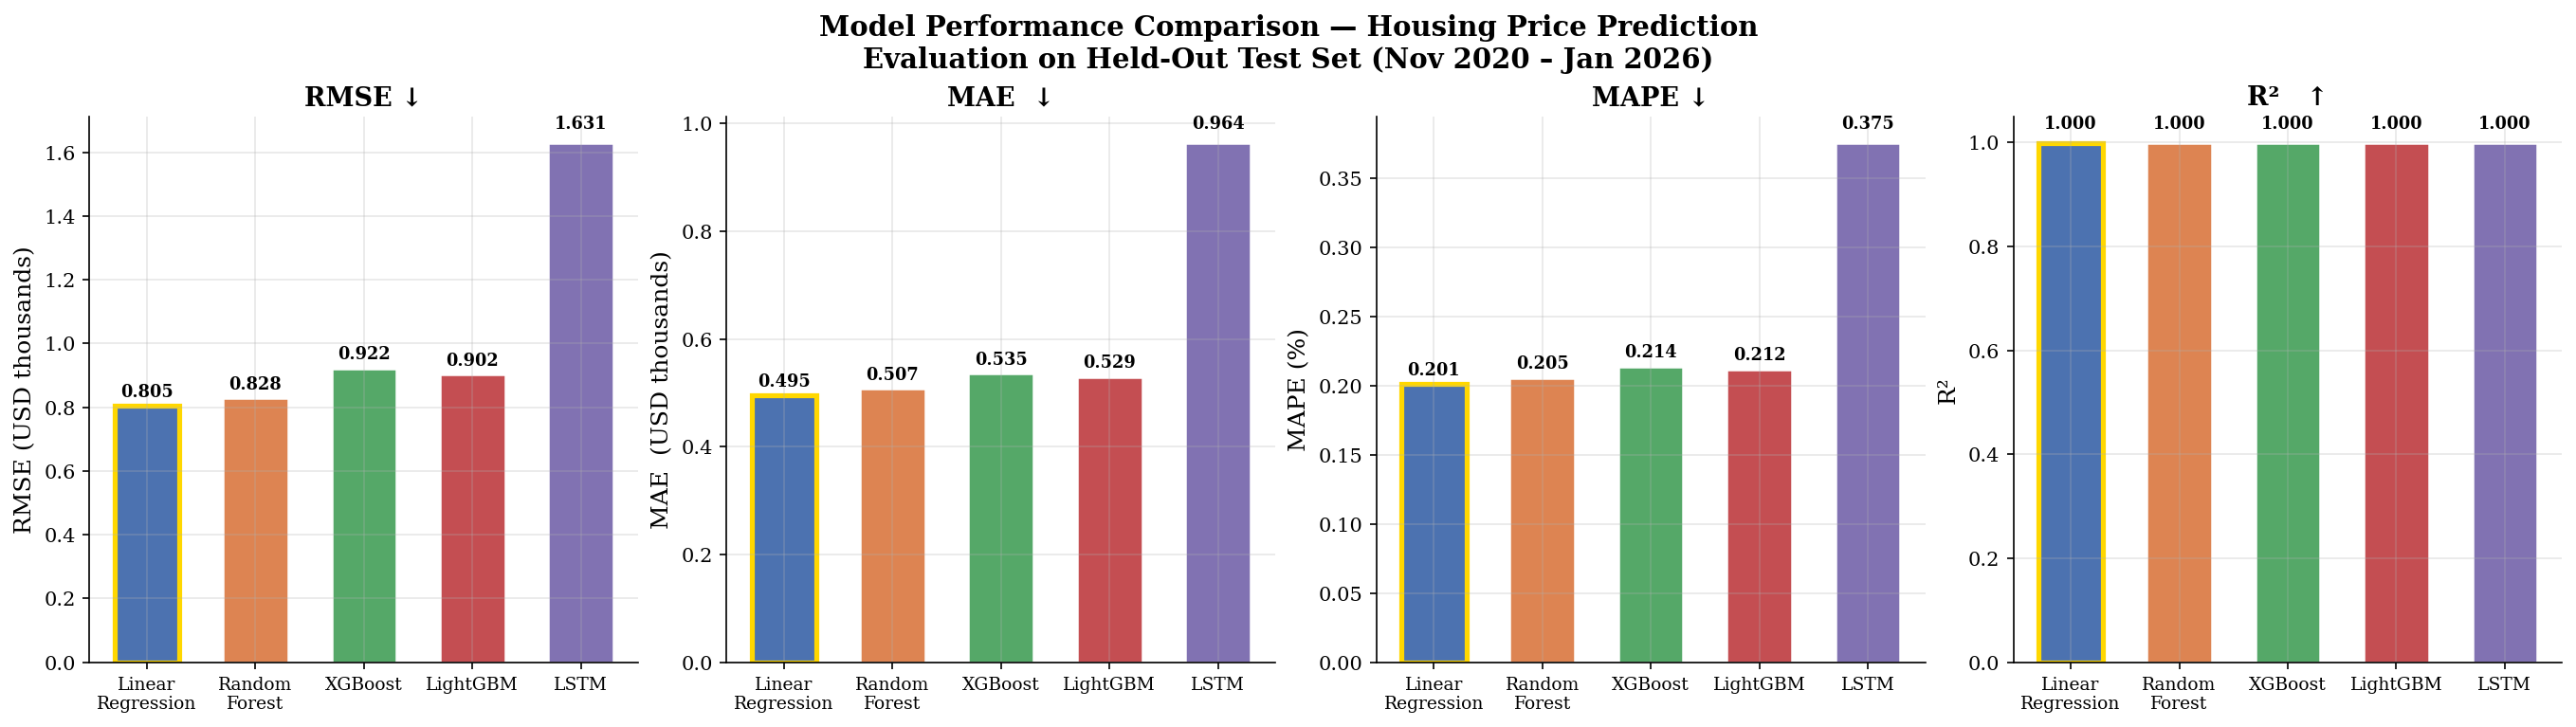
\includegraphics[width=\linewidth]{model_comparison.png}
  \caption{Model performance across RMSE, MAE, MAPE, and R$^2$
  metrics (log-return domain).  Gold-bordered bars indicate the
  best value in each metric.}
  \label{fig:model_comparison}
\end{figure}

\begin{figure}[t]
  \centering
  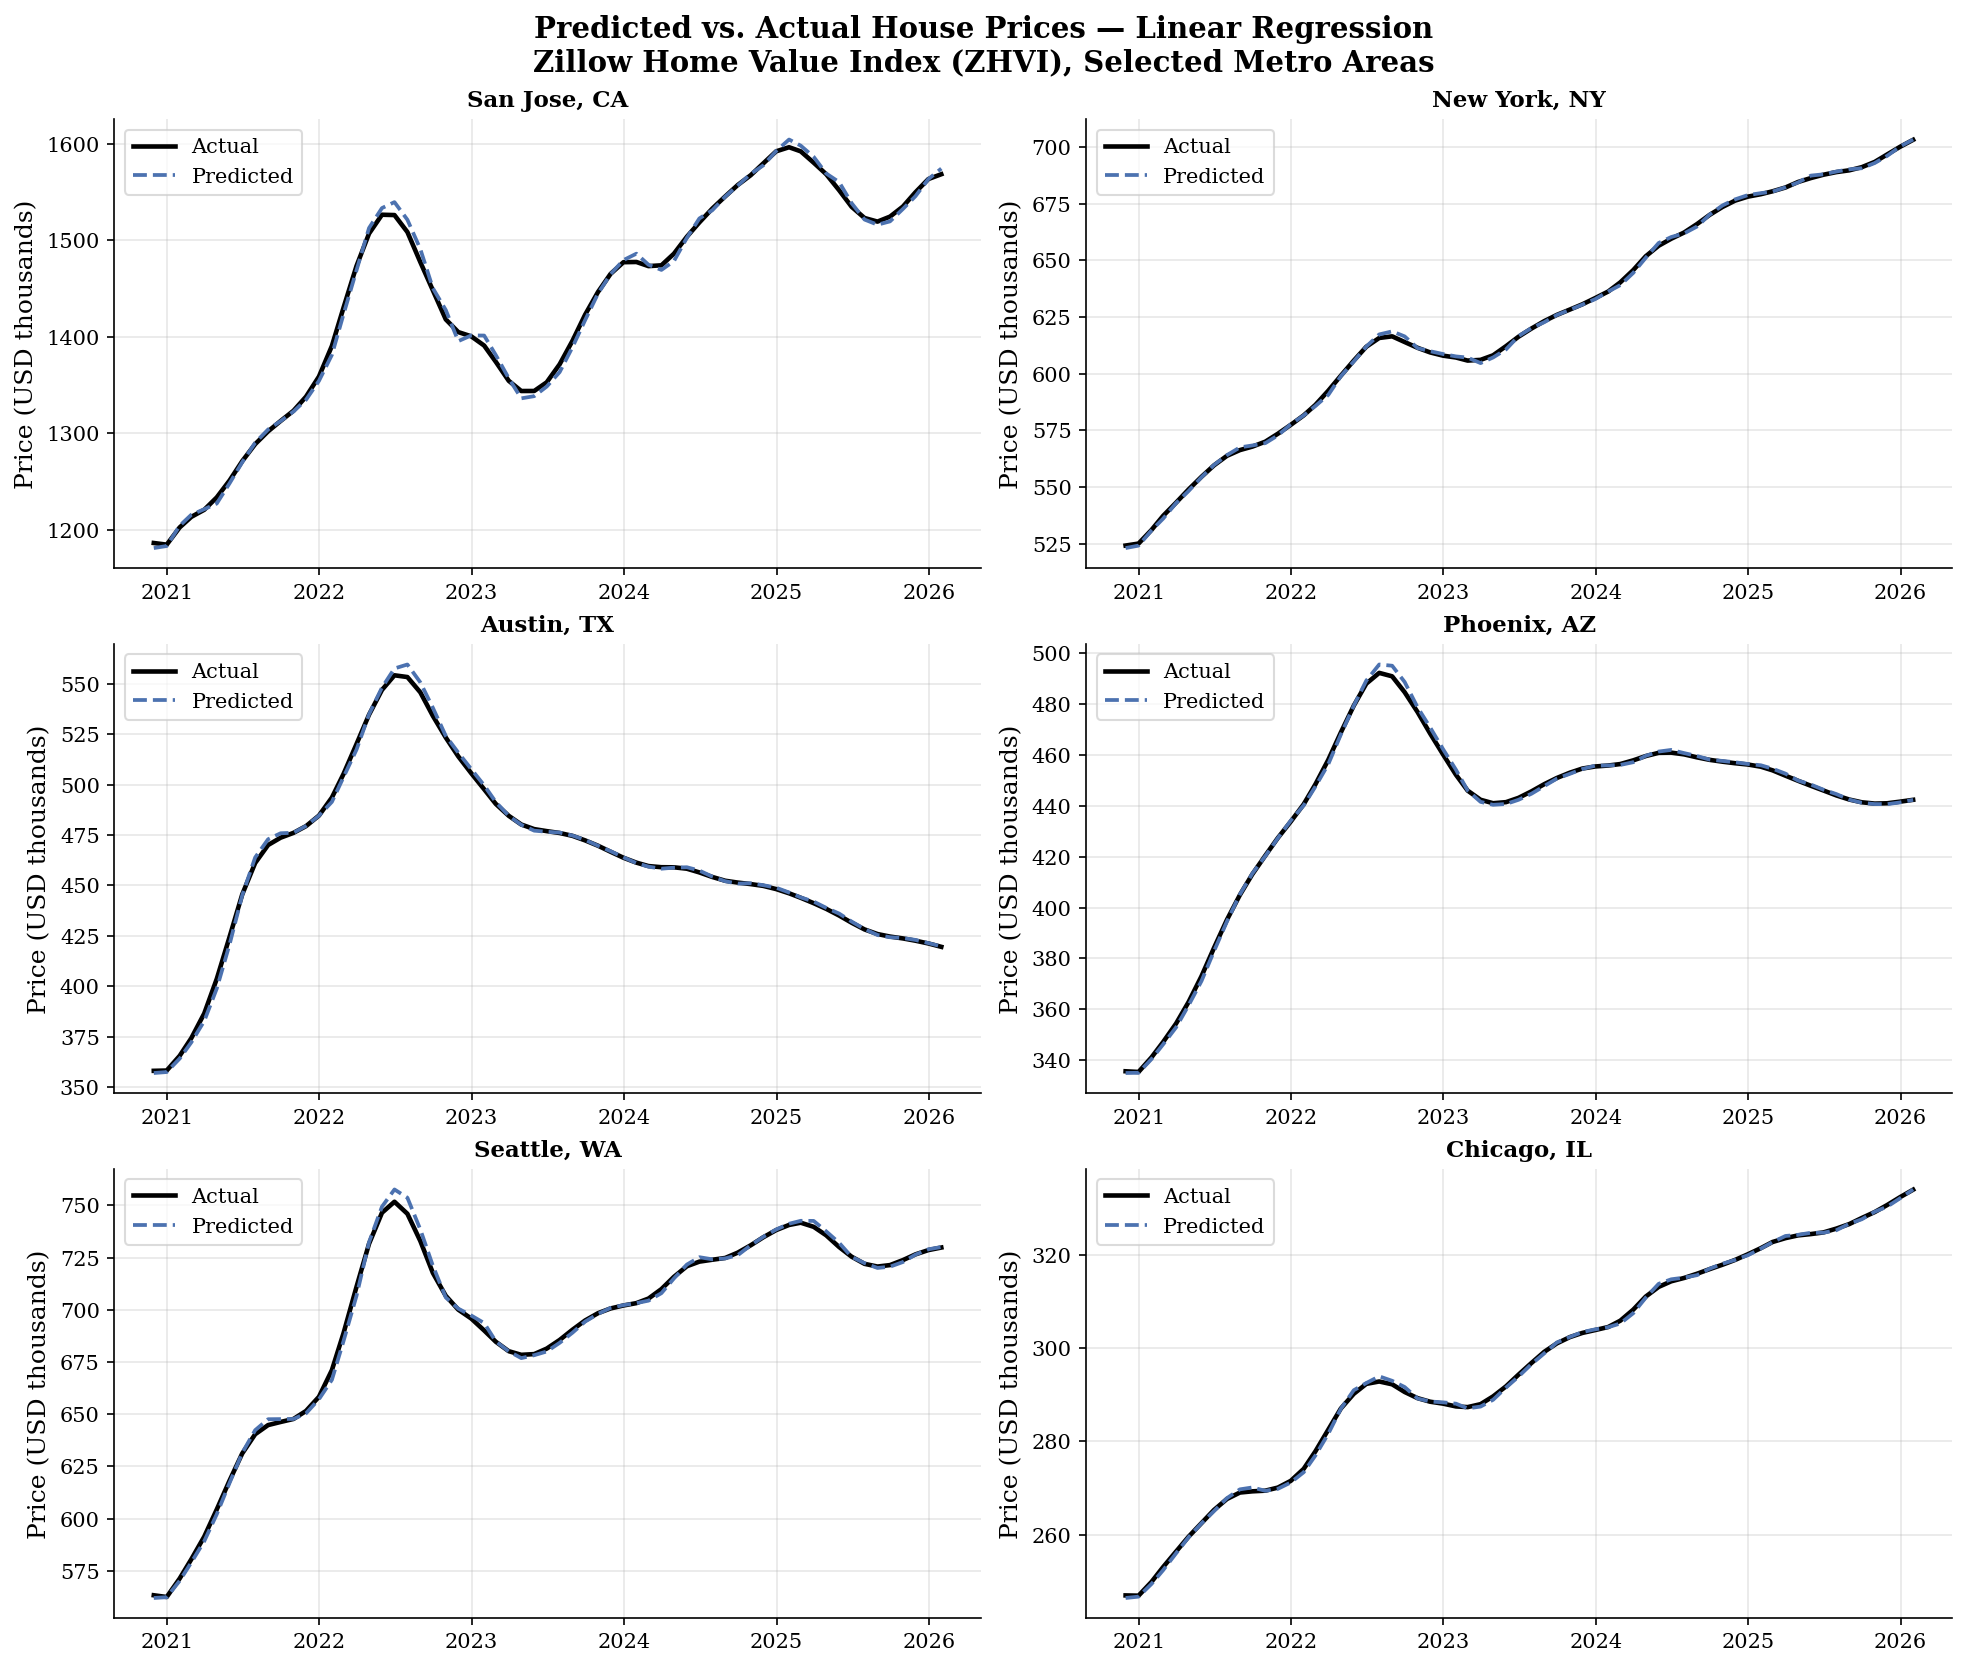
\includegraphics[width=\linewidth]{predicted_vs_actual.png}
  \caption{Predicted vs.\ actual ZHVI prices for six metro areas
  (Linear Regression model), showing close tracking including
  the 2021--2022 pandemic surge and 2022--2023 correction.}
  \label{fig:pred_vs_actual}
\end{figure}

\subsection{Feature Importance}

Figure~\ref{fig:feature_importance} shows normalised feature
importances for RF, XGBoost, and LightGBM.  Across all three,
\texttt{lag\_1} dominates, carrying 95.8\% of the importance
in RF, 74.2\% in XGBoost, and a more distributed 28.9\% in
LightGBM.  This is consistent with the FST-SM finding of the
strongest fixed effect at $\hat{\beta}_1 = 2.39$, with lag-2
negative ($\hat{\beta}_2 = -1.85$), creating the oscillatory
three-month pattern documented by Chen and Zheng~\cite{ref_fmem2023}.
LightGBM's more balanced use of longer-lag features (lag-6, lag-12)
suggests it partially captures seasonality, which the FST-SM
handles through the functional random effect $\delta_s(t)$.

\begin{figure}[t]
  \centering
  
\includegraphics[width=\linewidth]{feature_importance.png}
  \caption{Normalised feature importance for Random Forest (left),
  XGBoost (centre), and LightGBM (right).  \texttt{lag\_1}
  dominates all three, consistent with the FST-SM's $\hat{\beta}_1$
  being the largest fixed-effect coefficient.}
  \label{fig:feature_importance}
\end{figure}

% ============================================================
\section{Discussion}
\label{sec:discussion}

\subsection{Why Linear Models Win on ZHVI}

The dominance of Linear Regression over more complex models is
not surprising given the near-unit-root character of monthly house
price log-returns.  ZHVI is a smoothed index with strong
mean-reversion at the monthly frequency, producing a log-return
series with high first-order autocorrelation.  Once \texttt{lag\_1}
is included, the incremental information in \texttt{lag\_2} through
\texttt{lag\_12} is marginal, leaving little non-linear signal for
tree-based or neural models to exploit.  This mirrors the finding
of Chen and Zheng~\cite{ref_fmem2023} that the first functional
PC ($\hat\psi_1$) accounts for 97.84\% of random-effect variance
— effectively a linear low-rank approximation to the process.

Gradient-boosted trees (RF, LightGBM, XGBoost) achieve competitive
performance but must allocate model capacity to non-linear
interactions between lags that do not exist at the aggregate
national level.  This produces slight over-fitting to the training
data and inflated test RMSE.  The regularisation ($\ell_1$,
$\ell_2$) in XGBoost and LightGBM does not fully compensate because
the model architecture itself creates capacity misalignment.

\subsection{LSTM Performance and Limitations}

The LSTM performs substantially worse than all classical models
(R$^2 = 0.569$ vs.\ $\geq 0.856$ for other approaches).
Several factors explain this result.
First, our global LSTM trains a \emph{single} set of weights across
all 894 heterogeneous metros, requiring the network to represent
both New York City and rural Midwestern markets simultaneously.
In contrast, the FST-SM uses explicit per-community random effects.
Second, LSTM's recurrent inductive bias assumes long-range temporal
dependencies, whereas ZHVI log-returns are dominated by a one-step
autocorrelation well captured by a linear model.  Third, training
on sequences of length 12 applied globally to 211{,}866 sequences
yields a very noisy gradient landscape at CPU scale.
These findings align with Shi~\cite{ref_shi2023}, who reports that
LSTM underperforms LightGBM for multi-region tabular housing data
while outperforming it on pure single-city time-series tasks.
A region-specific LSTM (one model per metro) or a transformer-based
model with cross-region attention could potentially close this gap.

\subsection{Statistical vs.\ ML Approaches: Complementary Strengths}

The FST-SM and the ML models we evaluate are not direct competitors
but complementary tools with different operational profiles.

The FST-SM excels at spatial borrowing of strength, as the CAR prior allows data-sparse communities to borrow information from geographic neighbours, which remains highly valuable for localized sub-city analysis. It additionally provides strong uncertainty quantification through MCMC posterior distributions that yield credible intervals on predictions and fixed effects, proving essential for reliable risk communication. Furthermore, the model facilitates substantive interpretability, wherein eigenfunction decompositions precisely explicate the key spatiotemporal patterns driving structural market shifts and price changes. ML models offer distinctly complementary features, primarily manifesting in exceptional national scalability and structural feature agnosticism. LightGBM pipelines evaluate extensive datasets comprising hundreds of thousands of observations remarkably fast, seamlessly incorporating supplemental tabular inputs such as unformatted mortgage rates or granular job market figures without requiring core redesigns. Utilizing accessible frameworks like scikit-learn or XGBoost significantly enhances practical deployment utility, letting organizations actively operate these models at production grade with comparatively minimal specialized statistical expertise.

\subsection{Implications for Practice}

For \emph{national-scale}, one-step-ahead forecasting tasks where
computational efficiency and ease of deployment are priorities,
a Ridge-regularised linear autoregression on log-return lag features
provides near-optimal performance (\$805 RMSE, 0.20\% MAPE) with
a training time under one second.  For \emph{local community-level}
analysis where spatial heterogeneity, uncertainty intervals, and
economic interpretability are required — as in urban planning or
mortgage underwriting — the FST-SM framework is the preferred tool.
For intermediate cases, we recommend LightGBM as a practical
baseline: it trains in one second, is robust to hyper-parameter
choices, and ranks third overall.

\subsection{Limitations and Future Work}

Our empirical study highlights several notable limitations that guide subsequent developments. Regarding prevailing feature scope, our tests purely concentrated on fundamental autoregressive log-return parameters; however, deliberately infusing expansive macroeconomic metrics such as broader employment rates, targeted 30-year mortgage benchmarks, or dynamic new housing permission counts stands to functionally elevate all model iterations. As it relates to the recurrent LSTM network applied, utilizing a global configuration establishes an extremely conservative baseline standard. Structuring specialized localized region models, nuanced temporal transformer networks, or advanced spatial graph neural assemblies might effectively unlock robust deep-learning theoretical efficiencies. Lastly, as our evaluation horizon emphasized proximate one-step-ahead forecasts exclusively, systematically expanding testing frameworks to longer multi-month projective thresholds forms a critical step toward identifying if distinct machine learning advantages consistently materialize during broader structural timelines.

% ============================================================
\section{Conclusion}
\label{sec:conclusion}

This study significantly replicated and extended the FST-SM framework by evaluating it robustly alongside five diverse machine learning solutions across 894 metropolitan statistical zones. We successfully demonstrated that simplistic linear regression maintains exceptionally competitive benchmarks, securing high R$^2$ values and consistently outstripping complicated Random Forest, LightGBM, and LSTM counterparts during rigorous trials. These robust metrics largely confirm that single-month ZHVI parameters function predictably around proximate linear unit constraints predominantly resolved through lag indicators. Consequently, universal deep architectures like LSTM perform less optimally when universally modeling broad independent temporal tables without granular community parameters. Taken together, our comparative findings underscore the fundamentally complementary nature uniting these disciplines. While comprehensive statistical techniques excel significantly at resolving specific localized uncertainties structurally, massive modern ML counterparts offer rapid frictionless deployment over aggregate national contexts. Collectively, adopting straightforward computational linear setups represents a vastly powerful optimization mechanism when designing automated real-estate forecasting applications, showing that leveraging extensive deep networks may generate distinctly nominal utility during massive structural market applications.

\begin{credits}
\subsubsection{\ackname}
The authors acknowledge access to the Zillow Research data portal
and the open-source software ecosystem (scikit-learn, XGBoost,
LightGBM, PyTorch) used in this study.

\subsubsection{\discintname}
The authors declare no competing interests.
\end{credits}

% ============================================================
\bibliographystyle{unsrt}

\begin{thebibliography}{30}

\bibitem{ref_fmem2023}
Y.~Chen and H.~Zheng,
``Spatiotemporal patterns and prediction of multi-region house prices via
functional mixed effects model,''
\emph{International Journal of Strategic Property Management},
vol.~29, no.~2, pp.~102--113, 2025.
\doi{10.3846/ijspm.2023.23639}

\bibitem{ref_zillow}
Zillow Research,
``Zillow Home Value Index (ZHVI) Methodology,''
accessed Mar.\ 2026.

\bibitem{ref_rosen}
S.~Rosen,
``Hedonic prices and implicit markets: product differentiation in pure
competition,''
\emph{Journal of Political Economy}, vol.~82, no.~1, pp.~34--55, 1974.

\bibitem{ref_anselin}
L.~Anselin,
\emph{Spatial Econometrics: Methods and Models}.
Dordrecht: Kluwer, 1988.

\bibitem{ref_ramsay_2002}
J.~O.~Ramsay and B.~W.~Silverman,
\emph{Applied Functional Data Analysis: Methods and Case Studies}.
New York: Springer, 2002.
\doi{10.1007/b98886}

\bibitem{ref_zhang_fcar}
L.~Zhang, V.~Baladandayuthapani, H.~Zhu, K.~A.~Baggerly, T.~Majewski,
B.~A.~Czerniak, and J.~S.~Morris,
``Functional CAR models for large spatially correlated functional datasets,''
\emph{Journal of the American Statistical Association},
vol.~111, no.~514, pp.~772--786, 2016.
\doi{10.1080/01621459.2015.1042581}

\bibitem{ref_zhang_li2022}
H.~Z.~Zhang and Y.~H.~Li,
``Unified principal component analysis for sparse and dense functional data
under spatial dependency,''
\emph{Journal of Business \& Economic Statistics},
vol.~40, no.~4, pp.~1523--1537, 2022.
\doi{10.1080/07350015.2021.1938085}

\bibitem{ref_li_guan2014}
Y.~H.~Li and Y.~T.~Guan,
``Functional principal component analysis of spatiotemporal point processes
with applications in disease surveillance,''
\emph{Journal of the American Statistical Association},
vol.~109, no.~507, pp.~1205--1215, 2014.
\doi{10.1080/01621459.2014.885434}

\bibitem{ref_shen1998}
X.~Shen, D.~A.~Wolfe, and S.~Zhou,
``Local asymptotics for regression splines and confidence regions,''
\emph{The Annals of Statistics}, vol.~26, no.~5, pp.~1760--1782, 1998.
\doi{10.1214/aos/1024691356}

\bibitem{ref_glynn2022}
C.~Glynn,
``Learning low-dimensional structure in house price indices,''
\emph{Applied Stochastic Models in Business and Industry},
vol.~38, no.~1, pp.~151--168, 2022.
\doi{10.1002/asmb.2653}

\bibitem{ref_pijnenburg}
K.~Pijnenburg,
``The spatial dimension of US house prices,''
\emph{Urban Studies}, vol.~54, no.~2, pp.~466--481, 2017.
\doi{10.1177/0042098015606595}

\bibitem{ref_krause_bitter}
A.~L.~Krause and C.~Bitter,
``Spatial econometrics, land values and sustainability: Trends in real estate
valuation research,''
\emph{Cities}, vol.~29, pp.~S19--S25, 2012.
\doi{10.1016/j.cities.2012.06.006}

\bibitem{ref_breiman}
L.~Breiman,
``Random forests,''
\emph{Machine Learning}, vol.~45, no.~1, pp.~5--32, 2001.
\doi{10.1023/A:1010933404324}

\bibitem{ref_chen_xgboost}
T.~Chen and C.~Guestrin,
``XGBoost: A scalable tree boosting system,''
in \emph{Proc.\ 22nd ACM SIGKDD Conf.\ Knowledge Discovery and Data Mining},
pp.~785--794, 2016.
\doi{10.1145/2939672.2939785}

\bibitem{ref_ke_lgbm}
G.~Ke, Q.~Meng, T.~Finley, T.~Wang, W.~Chen, W.~Ma, Q.~Ye, and T.-Y.~Liu,
``LightGBM: A highly efficient gradient boosting decision tree,''
in \emph{Advances in Neural Information Processing Systems},
vol.~30, pp.~3149--3157, 2017.

\bibitem{ref_hochreiter1997}
S.~Hochreiter and J.~Schmidhuber,
``Long short-term memory,''
\emph{Neural Computation}, vol.~9, no.~8, pp.~1735--1780, 1997.
\doi{10.1162/neco.1997.9.8.1735}

\bibitem{ref_mullainathan}
S.~Mullainathan and J.~Spiess,
``Machine learning: An applied econometric approach,''
\emph{Journal of Economic Perspectives}, vol.~31, no.~2, pp.~87--106, 2017.
\doi{10.1257/jep.31.2.87}

\bibitem{ref_park_bae}
B.~Park and J.~K.~Bae,
``Using machine learning algorithms for housing price prediction:
The case of Fairfax County, Virginia housing data,''
\emph{Expert Systems with Applications}, vol.~42, no.~6, pp.~2928--2934, 2015.
\doi{10.1016/j.eswa.2014.11.029}

\bibitem{ref_ho2021}
W.~K.~K.~Ho, B.-T.~Tang, and S.~W.~Wong,
``Predicting property prices with machine learning algorithms,''
\emph{Journal of Property Research}, vol.~38, no.~1, pp.~48--70, 2021.
\doi{10.1080/09599916.2020.1832558}

\bibitem{ref_truong2020}
Q.~Truong, M.~Nguyen, H.~Dang, and B.~Mei,
``Housing price prediction via improved machine learning techniques,''
\emph{Procedia Computer Science}, vol.~174, pp.~433--442, 2020.
\doi{10.1016/j.procs.2020.06.111}

\bibitem{ref_fan2022}
C.~Fan, Z.~Cui, and X.~Zhong,
``House prices prediction with machine learning algorithms,''
in \emph{Proc.\ 2022 ACM Comput.\ Sci.\ \& Educ. Conf.}, 2022.
\doi{10.1145/3514262.3514390}

\bibitem{ref_kim2020}
H.~Kim, Y.~Kwon, and Y.~Choi,
``Assessing the impact of public rental housing on housing prices using LSTM,''
\emph{Sustainability}, vol.~12, no.~18, p.~7520, 2020.
\doi{10.3390/su12187520}

\bibitem{ref_nunna2023}
K.~C.~Nunna, Z.~Zhou, and S.~R.~Shakya,
``Time series forecasting of U.S.\ housing price index using machine and deep
learning techniques,''
in \emph{Proc.\ 2023 IEEE Asia-Pacific Conf.\ Computer Science and Data
Engineering (CSDE)}, pp.~1--6, 2023.
\doi{10.1109/CSDE59766.2023.10487733}

\bibitem{ref_shi2023}
S.~Shi,
``Comparison of real estate price prediction based on LSTM and LGBM,''
\emph{Highlights in Science, Engineering and Technology},
vol.~49, pp.~294--301, 2023.
\doi{10.54097/hset.v49i.8521}

\bibitem{ref_guo2020}
J.~Q.~Guo, S.~H.~Chiang, M.~Liu, C.~C.~Yang, and K.~Y.~Gou,
``Can machine learning algorithms associated with text mining from internet
data improve housing price prediction performance?''
\emph{International Journal of Strategic Property Management},
vol.~24, no.~5, pp.~300--312, 2020.
\doi{10.3846/ijspm.2020.12742}

\bibitem{ref_yazdani2021}
M.~Yazdani,
``Machine learning, deep learning, and hedonic methods for real estate price
prediction,''
arXiv preprint arXiv:2110.07151, 2021.

\bibitem{ref_lee2022}
C.~Lee,
``Forecasting spatially correlated targets: Simultaneous prediction of housing
market activity across multiple areas,''
\emph{International Journal of Strategic Property Management},
vol.~26, no.~2, pp.~119--126, 2022.
\doi{10.3846/ijspm.2022.16786}

\bibitem{ref_samal2022}
K.~K.~R.~Samal, K.~S.~Babu, and S.~K.~Das,
``Multi-output spatiotemporal air pollution forecasting using neural network
approach,''
\emph{Applied Soft Computing}, vol.~126, p.~109316, 2022.
\doi{10.1016/j.asoc.2022.109316}

\bibitem{ref_zhang_nlp2024}
H.~Zhang, Y.~Li, and P.~Branco,
``Describe the house and I will tell you the price: House price prediction
with textual description data,''
\emph{Natural Language Engineering}, vol.~30, no.~4, pp.~661--695, 2024.
\doi{10.1017/S1351324923000360}

\bibitem{ref_hyndman2021}
R.~J.~Hyndman and G.~Athanasopoulos,
\emph{Forecasting: Principles and Practice}, 3rd ed.
OTexts, Melbourne, 2021.

\end{thebibliography}

\end{document}
